\chapter{Evaluation}\label{C:evaluation}

\section{Objectives}

In this experiment, we aim to compare a latent factor approach to collaborative filtering with a hybrid collaborative filtering approach for the goal of ``Finding Good Items". The main objectives are to answer the following questions:
\todo{CHANGE: All these questions need to change}
\begin{itemize}
	\item{Can collaborative filtering provide personalised recommendaitons to users for the use case of ``Find Good Items"?}
	\item{What are the best variations of using like and dislike events for a latent factor CF approach}
	\item{Do using user preferences add value to collaborative filtering}
	\item{Is item similarity CF more accurate than user based for latent factor models}
	\item{Is hybrid CF more accurate than user based for latent factor models}
	\item{Is filtering recommendations by a black list more accurate for latent factor models}
	\item{Is filtering based on preferences of the user, more accurate for latent factor models}
\end{itemize}

\section{Design}

\todo{talk about an overview here?}
The goal of the experiment is to provide personalised food dish recommendations to users in regard to the ``Find Good Items" use case. A survey was given to participants capturing their food preferences and how they felt about specific food dishes. This data was used for an offline experiment to compare algorithms. We use use quantitative results from the survey to evaluate the performance of the algorithms in regards to the goal of ``Find Good Items". The quantitative results consist of the following evaluation metrics: accuracy, precision, recall, and precision at top N (10). These metrics are used in an offline experiment, however, an online experiment with the existing system should be conducted in future to validate the results. 
The following sections details the design of the experiment, the reasoning behind the metrics used, and the results. 

\subsection{Setup/Tools}
The following equipment was used to run the experiment:
\begin{itemize}
	\item{Intel(R) Core(TM) i7-4770 CPU @ 3.40GHz}
	\item{NVIDIA Corporation GM107GL 1gb graphics card}
	\item{\todo{DDR3 8gb RAM}}
	\item{Arch x86_64 GNU/Linux Operating System}
\end{itemize}

\subsection{Participants}

A total of 91 participants were involved in our experiment. Most participants were students from the school of Engineering and Computer Science from Victoria University. \todo{60} students from a first year Computer Science lecture and tutorial at Victoria University were involved in the experiment by filling out surveys capturing their food preferences and their opinions about food dishes. \todo{10} honours and masters students from Victoria University were asked to fill out our surveys. \todo{20} participants were from a Summer of Tech event that was held at Victoria University. The remaining participants were students from around the Computer Science labs at Victoria University.

The ages and gender were not captured of the participants due to drawbacks in the ethics process. It is estimated that most participants are students in the age range of 17-24 since most were recruited from the School of Engineering and Computer Science at Victoria University. There may be a minority of students that are over that age range. In addition, it is likely there are more male participants than female participants due to the location of recruitment. Participants were asked to fill out a survey.

\todo{vegetarian users, intolerant users, gluten free users, vegan users etc}

\subsection{Survey}

Qualitative data was collected from participants in the form of a survey. Participants were asked to rate their food preferences, their food intolerances, and their opinion about food dishes from the following likert scaled rating system: Hate, Dislike, Neutral, Like, and Love. Participants were asked to answer the Likert scaled ratings by circling the rating that best reflected their opinion of the food dish (See Figure \todo{figure number}). The survey contained 100 food dishes, \todo{10} food preferences, and \todo{intolerances} for participants to rate. Any unrated items were classified as Neutral ratings inferring participants had no opinion about the food dish or that they had not tried the food dish before. The survey was grouped into categories for participants to filter through the food dishes efficiently. All participants were shown the same food dishes but the ordering of the categories were randomised to help mitigate biases such as participants rating only the first items they see and so forth. All food dishes were captured from food vendors in the facility of Kelburn campus from Victoria University. Only the title of the food dishes were shown to participants, other information was excluded. This was to prevent biases around price, food vendor of where the food is given, and so on, which can influence the way participants rate the dishes. For example, a participant could like a food dish such as a chicken burger from one place, but hate a burger from another place. Other factors such as price affect the participants the way they rate the dish. Therefore, excluding this information allows us to capture the participants preferences of food in general, rather than specific dishes. \todo{Redo} (Doing this would be difficult as well and participants would get bored of the survey etc)

\todo{Show image}
No images were used to bias the results of the study. 
\todo{range of food dishes, i.e. vegan, vegetarian, intolerance}
\todo{portion of vegetarians etc}
A range of food was shown to participants ranging from gluten free, vegetarian, and vegan dishes. \todo{Fix this}

\subsection{Dataset}
In this section, we refer to a rating as a set of (u, i, r) triplets, where a user u has rated r on an item i. 
\todo{Should this go in dataset or survey section?}
The ratings collected from the survey consist of the following rating values: Hate (-1.0), Dislike (-0.5), Neutral (0.0), Like (0.5), Love (1.0). Since we are using Binary data only in the recommender system, we consider a like/love rating as a like event, and a dislike/hate rating as a dislike event in the algorithms. The reason why the granularity of like/love, and dislike/love were included in our survey in case we changed our minds on the types of events to use in the system.

The original data collected from the survey consists of the following:
\todo{put into table}
\begin{itemize}
	\item{100 food dishes}
	\item{91 users}
	\item{9100 total ratings}
	\item{\todo{18223 Like/Love ratings}} 
	\item{\todo{1000 Dislike/Hate ratings}}
	\item{\todo{7000 Neutral ratings}}
	\item{673 food preferences}
\end{itemize}

\todo{talk about SPARSITY \cite{zhang}}
% 
% The sparsity of a rating dataset is defined as the density of the vacancies in
% the user-item rating matrix, as in equation 2.1.
% sparsity = 1 −
% # ratings
% # users × # items
% (2.1)
% Because most users would have only rated a very small portion of the
% items, most recommendation datasets have very high sparsity, with sparsity
% as high as 0.95 considered normal [129].3 For this reason, in the field of
% recommender systems, the term “sparse” only refers to the extreme cases
% where the sparsity of the dataset is higher than 0.99. Such extreme sparsity normally occurs when new recommender systems are first established, or
% in datasets where the number of users is small relative to the volume of
% information in the system due to either a large number of items or regular
% updates of the item pool or both.

\todo{Add average Like and dislike ratings per user.}
\todo{Add min and max ratings of likes and dislikes from user?}
\todo{Add min,max,and average number of ratings for each item}
\todo{Talk about density in regards to user and item orientation of ratings}

\subsection{Data Cleansing}

The rating data of Like and Dislike events need to be fed through the algorithms to give personalised recommendations to users. The legitimacy of rating data provided will affect the way the collaborative filtering algorithms perform since it makes recommendations based on similar users. In order to mitigate this, we cleanse the data by removing participants that gave contradictory answers before we import the data in the recommender algorithms.

%  There were participants that had indicated they were vegetarians, but then had also indicated they had a preference for meat, rating meat dishes highly. This affects the recommendations that are shown by the algorithms.  

By examining the data collected from the surveys, it was evident that not all participants answered the questions legitimately. The most obvious were participants claiming to be vegetarian but had indicated they liked food dishes containing meat. Legitimate vegetarian users were easy to distinguish as they rated ``Hate" for every meat dish. There were other cases that were difficult to classify as legitimate. For example, a few participants specified they had intolerances to gluten, but indicated they liked eating food dishes with bread. This could mean several things such as participants having differing levels of tolerance to gluten, or perhaps the participants meant they liked eating the food dish with gluten free bread. Ambiguity in these cases meant we did not remove any participants we were unsure about. In addition, there were also cases where participants did not finish rating all items, and also participants that skipped pages in the survey. We included these users in the ratings for completeness as it enables us to see how the recommendation handles sparsity of ratings from these users. 

Overall, we removed users having contradictory answers refining the user data to the following dataset:
\todo{put into table}
\begin{itemize}
	\item{80 users}
	\item{8000 total ratings}
	\item{3937 Like/Love ratings}
	\item{1440 Dislike/Hate ratings}
    \item{2620 Neutral ratings}
	\item{613 food preferences}
\end{itemize}

\subsection{Overview}

To compare each algorithm to see which performs the best for our overall goal which is ``Find good items", we run an offline experiment. The method used in this experiment consists of partitioning the dataset, tuning the parameters, and validating the model using performance accuracy metrics. The following sections explain the details needed to understand the method in our experiment. We then state the method we used for comparing the different algorithms. 

\subsubsection{Data Partitioning}

To evaluate the recommender system algorithms in a standard offline evaluation, we partition the ratings dataset into a training set and a test set. The training set is used by the recommender algorithm to learn the model, and the test set is used to test the learned model to see how it performs on unseen data. In this case, the algorithms learn a model of user food dish preferences from the training set data, and use this to predict food dishes the users will like to which we then check against the test data. This is used to validate the generalisability of the model and gives an indication of how well it may perform in a real scenario, since the model has not seen the instances from the test data.

The skip-every-nth protocol \cite{zhang} is used to partition the dataset into a training set and a test set. The skip-every-nth protocol consists of randomising the ordering of users, and randomising the ratings within each user in a sequence that is contiguous, aggregating the result in a list sequence \cite{zhang}. The protocol iterates through this list of user ratings assigning every nth rating to the test set, the remaining ratings assigned to the training set. The skip-every-nth protocol ensures that ``the sparsity of the training dataset is minimally disturbed, and guarantees a (n - 1):1 size ratio between training and test data for all users up to decimal rounding" \cite{zhang}. However, since the nth value affects the user ratings that are involved in the test set, this means users with few ratings may not be in the test set since their ratings may be skipped during the process. 
\todo{Ask Sharon about this} In these cases, we evaluate the recommender algorithm n times with the same ordering, but offsetting the partitioning each run by 1. This ensures that every user rating is used exactly once in the test data \cite{zhang}. 

\todo{Should this be here?}
In our experiments, we use the skip-every-10th protocol as our partitioning technique for the final evaluation of the algorithm performance. We run the evaluation metrics multiple times with the optimal parameters and average the results. 

\subsubsection{Parameter Tuning}

Each algorithm has several parameters which influences the way it performs on final evaluation, hence the need to find the optimal parameters. To find the optimal parameters, we tune the parameters on the training set created by the skip-every-10th protocol and use k-fold cross validation. In this way, the test dataset remains uncontaminated since the optimised parameters have not been trained on the test data. 
We use standard 10-fold cross validation to determine the optimal parameters. In the context of this project, the goal of k-fold cross validation is used to determine a model with optimised parameters during the training phase which will limit problems of over-fitting. 

\todo{May need to reexplain this. difficult to understand?}
The technique used to find the optimal parameters is k-fold cross validation. K-fold cross validation consists of partitioning the dataset, in our case, the training set into k equal sized subsets. We randomise the training set before partitioning the set into k subsets. A subset from the k subsets is then selected as the validation data, and the remaining subsets (k-1) are used as the training data. Evaluation metrics are then calculated. This is repeated k times where each subset is used as the validation subset exactly once, and the results from the metrics are averaged to determine how good the parameters are for that run. This process is then repeated multiple times with different parameters, the optimal parameters being chosen for the final evaluation. K-fold cross validation was chosen as it considers the variance in the data by averaging the results, and uses each data point exactly once, mitigating results the likelihood of lucky one-off results. In addition, it reduces the likelihood of overfitting. 

\subsubsection{Recommendation Accuracy}

In the context of recommender systems, recommendation accuracy measures the performance of a recommender system based on how well the system can correctly distinguish whether a user will like an item or whether they will not. This is similar to the decision end users make in a real world scenario where decisions are based on binary recommendations such as acceptance or rejection \cite{zhang}. Therefore, recommendation accuracy metrics are appropriate for the use case of ``Find Good Items" \cite{evaluation}. Therefore, we use recommendation accuracy as a metric since our goal is to ``Find Good Items".\todo{figure out where to put this} For recommendation algorithms that output rating predictions, a threshold-cutoff is used to determine is used to determine the good items from the bad items \cite{zhang}.

However, there are caveats to using recommendation accuracy. Recommendation accuracy does not measure the quality of the items recommended as it does not measure the ability of an algorithm to accurately predict ratings, thus, does not focus on the correct ordering of the recommendations list based on the users preference of items. \todo{clarify this, may need to explain more such as deviations etc. Also top-N is not our use case... users could get bored after awhile. we don't care about ranking as long as users like the recs.}. This also means that it does not guarantee the user will see all the liked items in the top-N recommendations list. In addition, recommendation accuracy is identifying items that the user is already aware of, which makes it susceptible to biases involving overfitting and non-novel recommendations \cite{evaluation}. 

For these reasons, we use recommendation accuracy with supporting metrics of precision, recall, and precision at N. 

\subsubsection{Precision, Recall, and Precision at N}
\todo {Should I use all of these? Precision of the whole test data? Recall of the whole dataset? or just precision @ N?}

Binary recommendations can fall into one of four categories. \todo{TP, FP, TN, FN - Show table. Expand on this}

For binary ratings, precision and recall are often used as metrics. Precision measures the relevant recommendations (fidelity) to the user \todo{add equation for precision}, whereas Recall measures the relevant recommendations from the total preferred items (completeness) \todo{add equation for recall}. 

Precision at N looks at the top recommendations list, and sees how many true liked items are in that list, and how many false liked items are not in the list. This can be used to measure the portion of relevant items that are in the top-N recommendation list.

% Recall, in its purest sense, is almost always impractical to measure in a
% recommender system. In the pure sense, measuring recall requires knowing
% whether each item is relevant; for a movie recommender, this would involve
% asking many users to view all 5000 movies to measure how successfully we recommend
% each one to each user

% Perhaps a more appropriate way to approximate precision and recall would
% be to predict the top N items for which we have ratings. That is, we take a
% user’s ratings, split them into a training set and a test set, train the algorithm
% on the training set, then predict the top N items from that user’s test set. If we
% assume that the distribution of relevant items and nonrelevant items within
% the user’s test set is the same as the true distribution for the user across all
% items, then the precision and recall will be much closer approximations of the
% true precision and recall. This approach is taken in Basu et al. [1998].
% In information retrieval, precision and recall can be linked to probabilities
% that directly affect the user. If an algorithm has a measured precision of 70%,
% then the user can expect that, on average, 7 out of every 10 documents returned
% to the user will be relevant. Users can more intuitively comprehend the meaning
% of a 10\% difference in precision than they can a 0.5-point difference in mean
% absolute error

% One of the primary challenges to using precision and recall to compare different
% algorithms is that precision and recall must be considered together to
% evaluate completely the performance of an algorithm.

% Precision alone at a single search length or a single recall level can be appropriate
% if the user does not need a complete list of all potentially relevant
% items, such as in the Find Good Items task. If the task is to find all relevant
% items in an area, then recall becomes important as well. However, the search
% length at which precision is measured should be appropriate for the user task
% and content domain.

\subsubsection{ROC Curves}
\todo{redo}
In the context of this project, Receiver Operating Characteristic (ROC) curves are used to visualise all the possible thresholds on a graph displaying how well a model is able to distinguish recommendations that the user will like or dislike. The True Positive (TP) rate which is the y-axis, shows the sensitivity of the model. This means that it shows the fraction in which liked items by specific users are correctly recommended to the users. The False Positive (FP) rate which is the x-axis, shows the fraction in which disliked items by specific users are incorrectly recommended as items they would like. 

\subsubsection{Area Under The Curve}
\todo{Explain this}


\subsection{Method}

\todo{Rewrite all of this. Just check if content is correct.}

The method focuses on two cases. The first focus is finding the optimal parameters for each algorithm to finalise the algorithm that performs best. This will be used for future prediction in an online-study or real scenario to see how real users will respond to each algorithm. The next focus is to compare which algorithm performs the best in an offline evaluation, and in the context of this project.

For the first method, we use the skip-every-10th protocol to obtain a training set and a test set. Using only the training set, we find the optimal parameters for an algorithm by performing 10-fold cross validation. Since cross-validation uses each subset as validation data, we retrain the model on the whole training set data with the optimal parameters obtained from the k-fold validation. Using this model, we run it 30 times on the test set computing the recommendation accuracy, the precision, the recall, and the precision at N (10). The results are then averaged over the 30 runs. 

\todo{Check this} Each different run uses the skip-every-10th protocol with an offset, so every test point is used exactly once. This method should give an optimal tuned parameters for future prediction used to finalize the system, however, contains biases in the test data. For these reasons, we do the second method to compare the algorithms, since the test set will not be contaminated with data from the tuning phase.

The second method is essentially the same as the first, except we tune the parameters each run to get the best results. In this way, the test data is uncontaminated and we can use this to compare the different algorithms when they perform at their best. However, this method means that the parameters are not finalized, hence why we do the first method. 

% 1) tune the parameters using the whole data set and then do the normal leave-n out training and testing. (this is what Bing suggested) The parameters are tuned and they are finalized. But the testing has bias because some testing cases might be used in tunning. This method is good to finalize a system so it can be used for future prediction.

% 2) k-fold, for each round, you do training, tuning and testing, so you split the data into three parts. Using this method, the parameters are tuned for each round(you do the tuning for k times), so they are not finalized, so it is not good for predicting, but the testing has no bias.

\section{Experimental Results}

In this section we present the results of the experiments described in Section \ref{Method}. In Section 5.1, we will focus on comparing the hybrid CF approach to the standard ALS CF approach, demonstrating the use of food dish content used inside the hybrid CF technique is able to outperform the standard CF ALS approach. This section also demonstrates the optimal parameters for the different approaches for further investigation in a commerical/real world environment.  

\begin{figure}
\centering
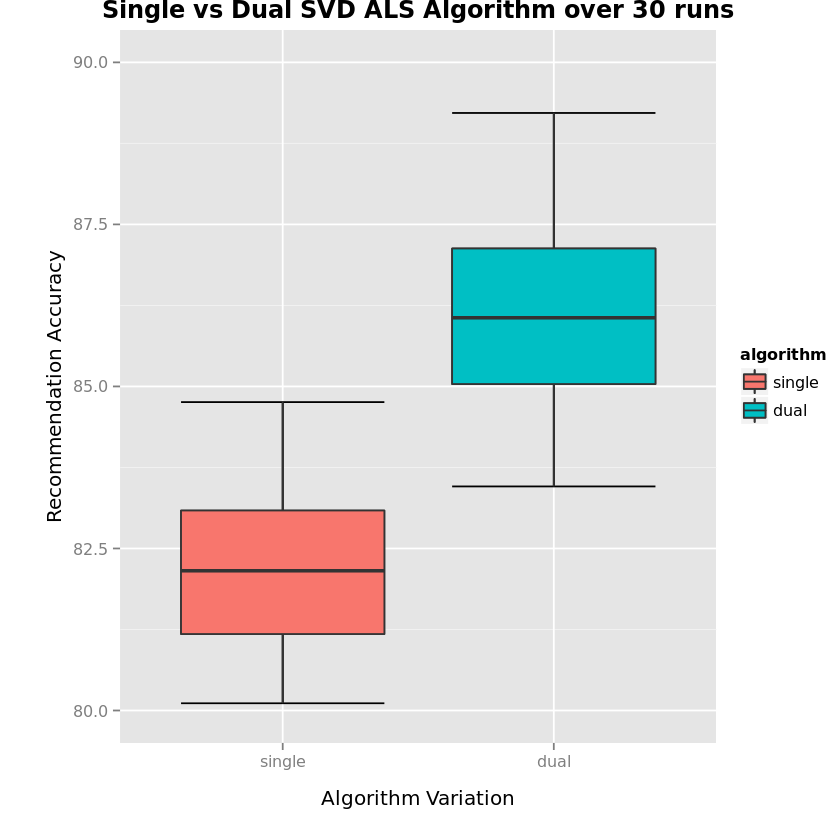
\includegraphics[scale=0.7]{images/single_vs_dual.png}
\caption{Recommendation Accuracy from variation of ALS algorithm ran 30 times.}
\label{fig:algorithms}
\end{figure}


\begin{figure}
\centering
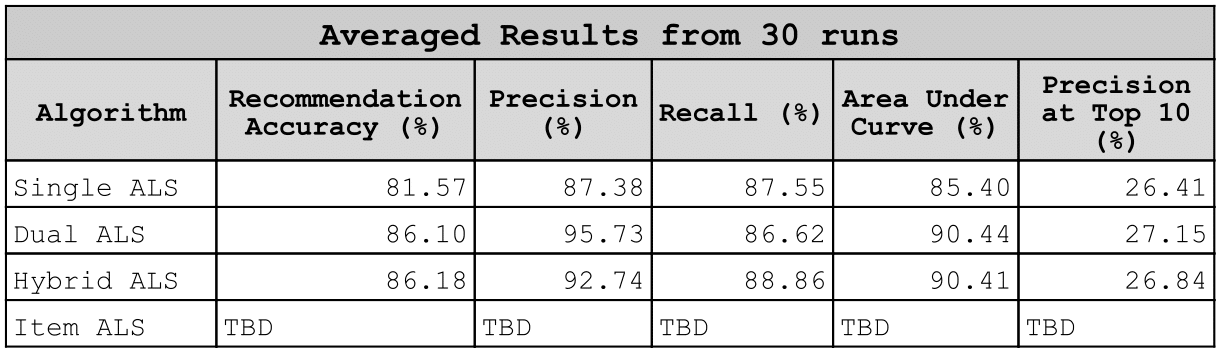
\includegraphics[scale=0.4]{images/results_tuning.png}
\caption{Averaged results ran 30 times with the same optimal parameters (contaminated).}
\label{fig:results}
\end{figure}

\begin{figure}
\centering
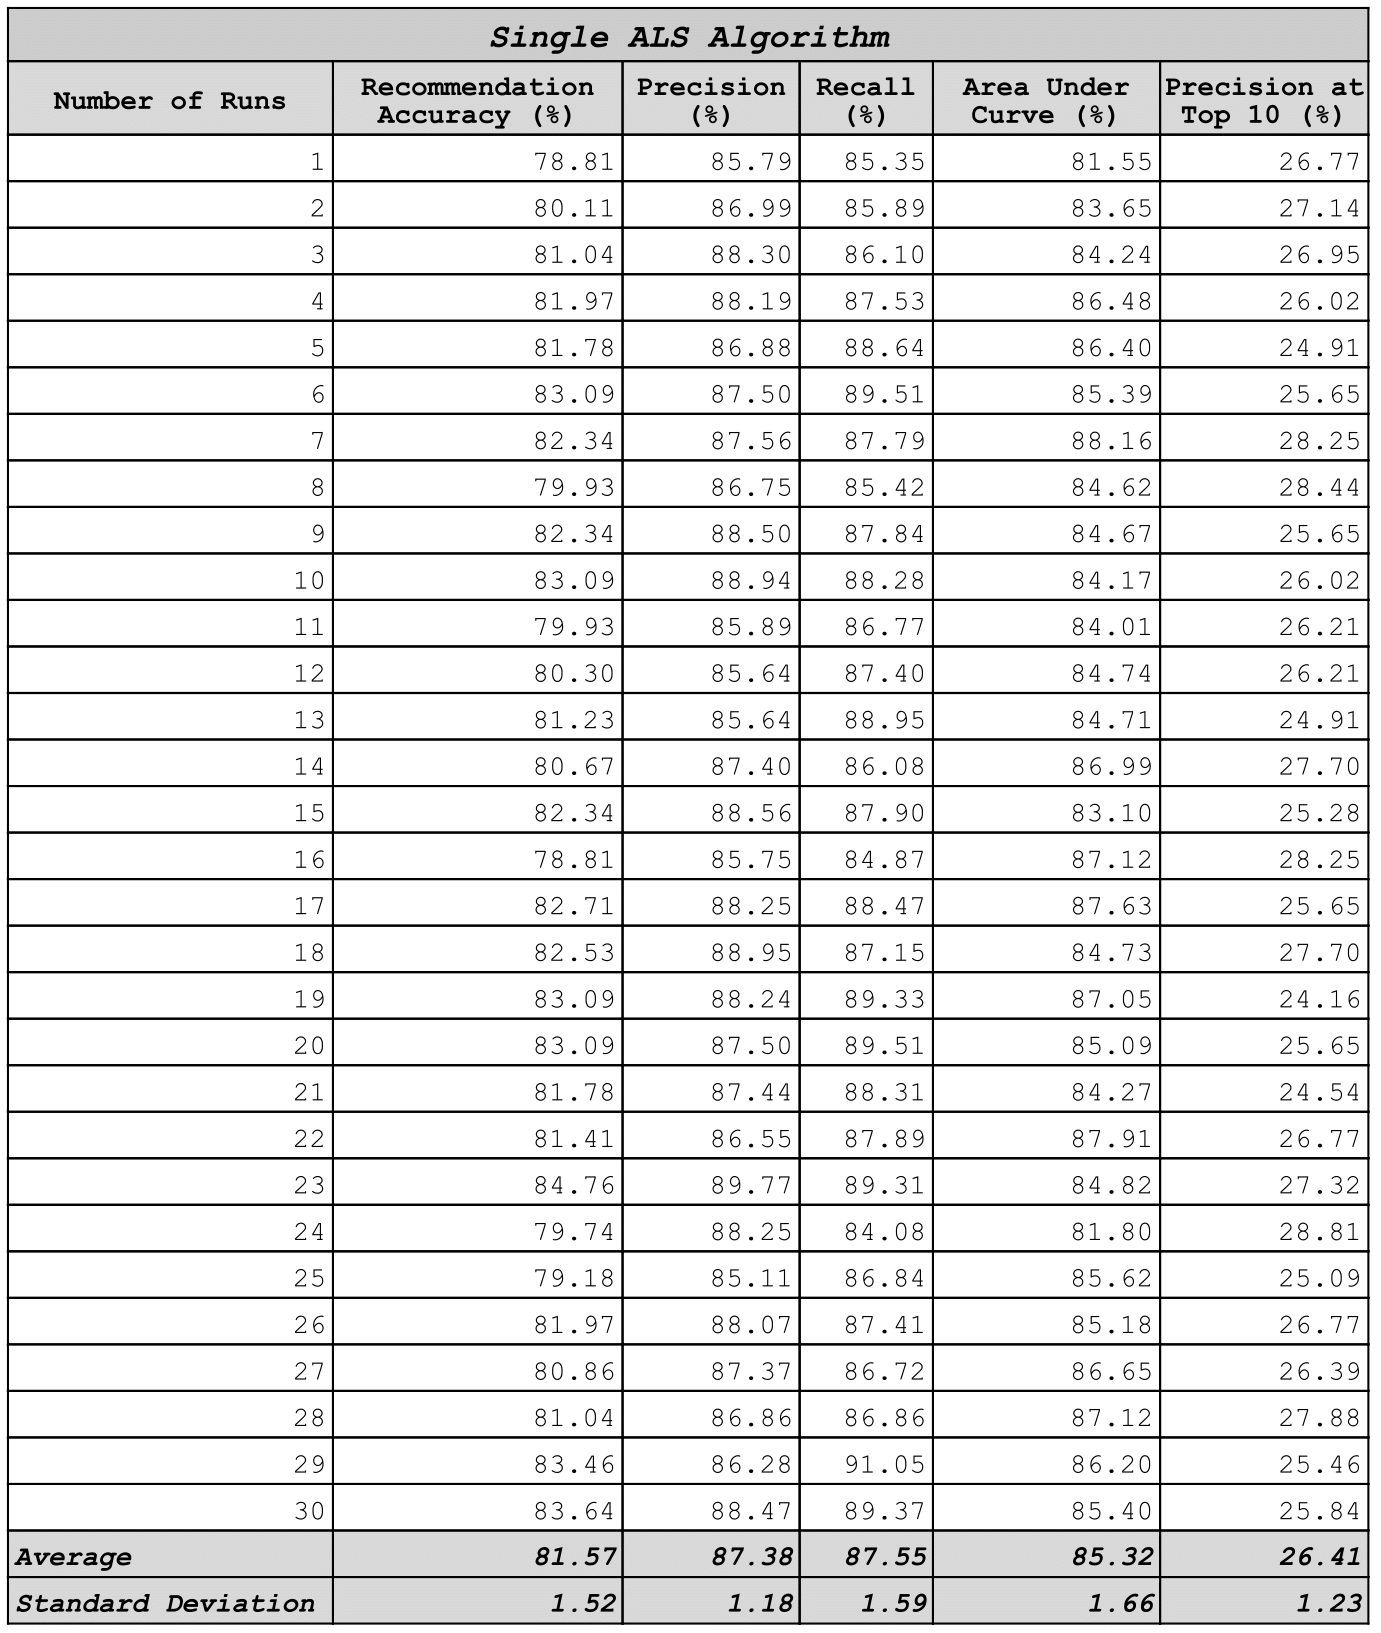
\includegraphics[scale=0.3]{images/single_als_30_runs.png}
\caption{Individual 30 runs of the standard single ALS algorithm. (contaminated)}
\label{fig:single_algorithm}
\end{figure}

\todo{Check this - massive Brain dump to get content down (probably wrong as well)}
From running these algorithms multiple times, it is clear that the results give similar results. 

\subsection{Recommendation Accuracy}
Recommendation accuracy is the most suitable for the use case of ``Find Good Items". From the results, the hybrid collaborative filtering seems to provide the highest accuracy in this case. The preferences from each user describing the attributes the user likes and dislikes, provides extra information to the recommender system, thus resulting in the higher accuracy. However, this information may not be available. \todo{Hybrid achieved x accuracy}. The dual algorithm was able to provide more accurate predictions than the single algorithm. This validates objective \todo{do this} where the dual algorithm was able to correlate the events of likes and dislikes better than use of the single algorithm.

\subsection{Precision}

\subsection{Recall}

\subsection{Precision at top N (10)}


\section{Analysis}
\todo{TAKE THIS OUT?}
\subsection{Parameter Tuning}
\todo{Not sure if this should be included? Usually in reports they do something like this?}

\subsection{\todo{Latent size}}
\todo{directly from design decisions}
\todo{Should I include stuff like this in the report?}
This affects the amount of features that will be used in SVD.

With the current amount of data, it seems that using a smaller latent size affects the accuracy. This is because having a smaller latent size will capture all the ``Strong" patterns from the ratings, as opposed to having a larger number of latent sizes, where the rating patterns are spread across more characteristics, meaning that the feature values for these characteristics will be smaller. More feature vectors -> the smaller the strength of the characteristics that it captures from the previous rating patterns. This may capture quirky characteristics from the users rating patterns...however, Less feature vectors -> the stronger the strength of the characteristics that it captures from the previous rating patterns. 

% \subsection{\todo{Implicit events}}
% \todo{directly from design decisions}
% Seems like it can’t recognize negative values
% Using the implicit training is not able to classify negative values. 
% If you look at the values where the actual values were either hate or dislike, then all the predicted values are positive. This may be caused by the ratings of others on the dish.
% If we look at the data, It is skewed. There are far more likes/loves than dislikes/hates. This may cause the values in the item feature vectors and user feature vectors to all be positive, since all the positive ratings are overpowering the negative values. For instance, a user’s predicted score is reliant on the value of the item feature vector and the user’s feature vector of tastes. The cross product determines the user’s preference for the item. If many other users have rated the item being liked than disliked, then this will positively impact the feature values of the item feature vector such that the negative values are not even considered. 
% This may also affect the classification accuracy because all the predicted rating dishes are going to be based on positive ratings, meaning that the evaluation may be inaccurate. For instance, since all the item vectors are overpowered by positive ratings, then all the instances in the test set where the user has indicated that they “like/love” the dish will also be positive. This leads to biased results since every dish is positive within a threshold. 
% To resolve this, we may have to compute two engines, for likes and dislikes. 
% Also the cause of this may be because we are not training with explicit ratings.


\section{Limitations}
% \cite{martin2009recsys}
% Examples of this problem
% include the lack of standard treatment of items for which
% the recommender is unable to make a prediction. The broader
% goal of user-centered holistic evaluation, including A/B testing
% of the short- and long-term effects of recommendation differences,
% is still met by only a few research groups and companies
% that have the live systems and resources for such evaluation.

% Deploying innovative recommenders is still too hard, and there is a substantial need for research platforms where innovations can be tested without first building up a community of thousands of users. 
\todo{Write this whole section}
\todo{Rewrite all of these points into sentences}
\begin{itemize}
	\item{Offline experiment may not be enough, users may feel different}
	\item{Contradictions in the data and participation}
	\item{Proportion of items and user}
	\item{The labelling of data, removing the location, price etc}
	\item{The amount of users, and the amount of ratings, and the amount of items. Variety of food choices for vegans etc. }
	\item{The participants recruited - need to be more generalised (Mainly from students)}
	\item{Tuning the parameters? or unbiased datasets}
	\item{Online evaluation - novelty, serependity, etc, how can users give opinions about items they've never tried before}
	\item{Density and sparsity of the matrix}
	\item{The survey questions - need to ask the right questions and about how you ask the question.}
\end{itemize}
\todo{From design decisions}
Not enough representation of vegans or vegetarians
Not enough vegetarian or vegan dishes. 
This may cause recommendations to be minimal etc.
Also meat lovers may overpower the items?
Noticed that Vegetarians all rated items with meat as “HATE” this could affect the overall predictions for SVD?
May not be linearly separable?
People may not fill in survey correctly.
Some people may have filled out dishes that they haven't tried before. This could affect the results because often what people do is different to what they think. 
There were cases where people filled out the form inaccurately, such that they chose random dishes. We know this because there are cases where someone states that they are “vegetarians” but then say they like “meat” etc.
Cleanse these cases to give better predictions

\section{Discussion}


% \section{\todo{Offline evaluation}}
% OFFLINE EVALUATION
% \todo{directly from design decisions}
% Offline evaluation does not determine whether users will like novel items or not. We cannot possibly measure this, since there are a vast amount of missing ratings from the users. 
% With an offline evaluation, we can only test against what the users have rated. Therefore, we cannot really test the novelty factor, as we can’t know if the user will like the top n list of recommendations since many will be missing. For this, we can use precision and recall but it means that the result will be dependent on the amount of rated positive items the user has done, and how many appear in the list. For this reason, there will be many FALSE POSITIVES, because users have not rated this item. 
% Therefore, an ONLINE evaluation would be the best to get a gauge on how the users really feel about the recommendations. There are a couple factors that are needed for this:
% A real system
% Users will have needed to rate a number of items
% There must be a vast amount of already rated items in the system
% Some users may not tried dishes so may not be able to label it accurately?




